\begin{Example}
\label{ex:sturm-liouville-robin-example}
考虑由微分方程
\begin{equation}\label{eq:sturm-liouville-robin-example-ode}
-u''-\lambda u=0
\end{equation}
和边界条件
\begin{equation}\label{eq:sturm-liouville-robin-example-left-condition}
u(0)=0,
\end{equation}

\begin{equation}\label{eq:sturm-liouville-robin-example-right-condition}
\cos\beta\,u(1)+\sin\beta\,u'(1)=0.
\end{equation}
组成的 Sturm-Liouville 特征值问题. 不失一般性, 假设 $-\pi/2<\beta\leq\pi/2$.

例如, 对一个描述细长杆的一维热传导问题作分离变量, 就会得到这一方程. 杆的侧面绝热, 一端保持固定温度, 另一端向外辐射热量.

根据 $\lambda$ 的符号, 得到 \eqref{eq:sturm-liouville-robin-example-ode} 的以下双参数实解族:
\begin{equation}\label{eq:sturm-liouville-robin-example-general-solutions}
y(x)=\begin{cases}
A\cosh\sqrt{-\lambda}x+B\sinh\sqrt{-\lambda}x,&\lambda<0,\\
A+Bx,&\lambda=0,\\
A\cos\sqrt{\lambda}x+B\sin\sqrt{\lambda}x,&\lambda>0.
\end{cases}
\end{equation}
应用边界条件 \eqref{eq:sturm-liouville-robin-example-left-condition}, 得到
\begin{equation}\label{eq:sturm-liouville-robin-example-left-reduced-solutions}
y(x)=\begin{cases}
B\sinh\sqrt{-\lambda}x,&\lambda<0,\\
Bx,&\lambda=0,\\
B\sin\sqrt{\lambda}x,&\lambda>0.
\end{cases}
\end{equation}
现在分析第二个边界条件.\begin{enumerate}\item 当 $\lambda<0$ 时, 令 $\omega=\sqrt{-\lambda}$. 那么 \eqref{eq:sturm-liouville-robin-example-right-condition} 变为
\begin{equation}\label{eq:sturm-liouville-robin-example-negative-boundary-equation}
B(\cos\beta\sinh\omega+\omega\sin\beta\cosh\omega)=0.
\end{equation}
\begin{figure}[H]
\centering
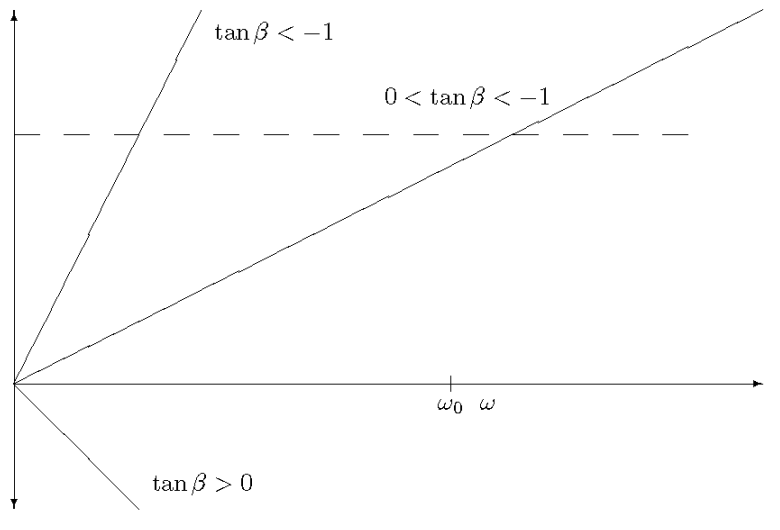
\includegraphics[width=.78\linewidth]{figures/sturm-liouville-negative-spectrum-source.png}
\caption{下式的解: $\tanh\omega=-\omega\tan\beta$.}\label{fig:sturm-liouville-negative-roots}
\end{figure}注意, 若 $\beta=\pi/2$, 则无解. 因而存在非平凡解, 当且仅当存在满足下式的 $\omega>0$:
\begin{equation}\label{eq:sturm-liouville-robin-example-negative-root-equation}
\tanh\omega=-\omega\tan\beta.
\end{equation}
由 Figure~\ref{fig:sturm-liouville-negative-roots} 可见, 若 $\tan\beta\in(-1,0)$ (即 $\beta\in(-\pi/4,0)$), 则恰有一个解 $\omega_0$, 否则无解. 若解存在, 则它对应于特征值 $\lambda_0=-\omega_0^2$ 和特征函数 $u_0(x)=\sinh\omega_0x$.\item 当 $\lambda=0$ 时, \eqref{eq:sturm-liouville-robin-example-right-condition} 变为
\begin{equation}\label{eq:sturm-liouville-robin-example-zero-boundary-equation}
B(\cos\beta+\sin\beta)=0.
\end{equation}
因而存在非平凡解, 当且仅当 $\beta=-\pi/4$. 此时 $\lambda_0=0$ 是特征值, $u_0(x)=x$ 为相应特征函数.\item 当 $\lambda>0$ 时, 令 $\omega=\sqrt{\lambda}$. 那么 \eqref{eq:sturm-liouville-robin-example-right-condition} 变为
\begin{equation}\label{eq:sturm-liouville-robin-example-positive-boundary-equation}
B(\cos\beta\sin\omega+\omega\sin\beta\cos\omega)=0.
\end{equation}
对于 $\beta\in(-\pi/2,\pi/2)$, 存在非平凡解, 当且仅当存在满足下式的 $\omega>0$:
\begin{equation}\label{eq:sturm-liouville-robin-example-positive-root-equation}
\tan\omega=-\omega\tan\beta.
\end{equation}
\begin{figure}[H]
\centering
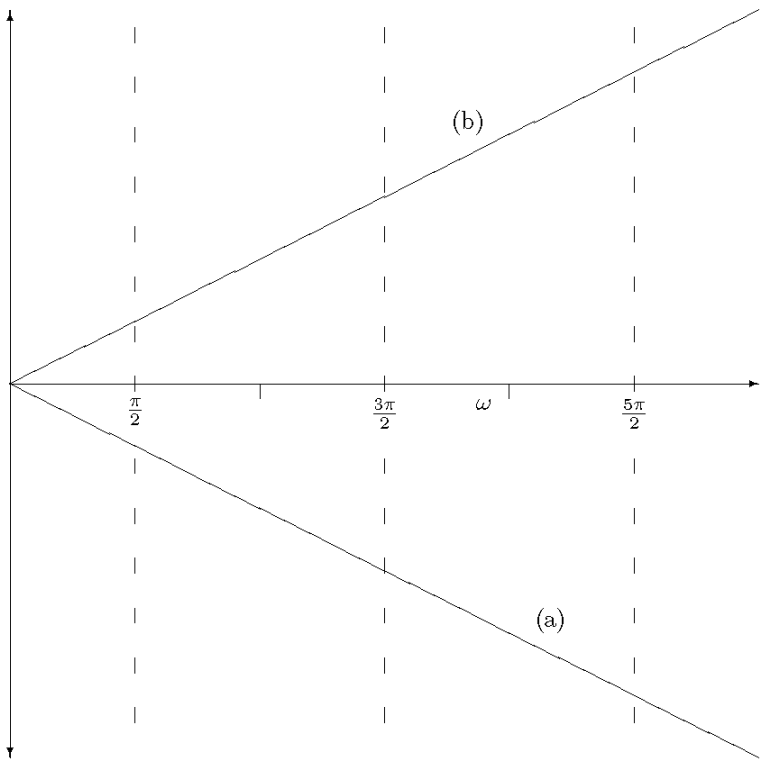
\includegraphics[width=.78\linewidth]{figures/sturm-liouville-positive-spectrum-source.png}
\caption{下式的解: $\tan\omega=-\omega\tan\beta$. (a) $\tan\beta>0$. (b) $\tan\beta<0$.}\label{fig:sturm-liouville-positive-roots}
\end{figure}由 Figure~\ref{fig:sturm-liouville-positive-roots} 可见, 对任意 $\beta\in(-\pi/2,\pi/2)$, 此方程有无穷解族 $\omega_n$, $n=1,2,3,\ldots$, 且 $\lim_{n\to\infty}\omega_n=\infty$. 因而存在无穷特征值族 $\lambda_n=\omega_n^2$, 相应的特征函数为 $u_n(x)=\sin\omega_nx$, $n=1,2,3,\ldots$.

若 $\beta=\pi/2$, 则直接解 \eqref{eq:sturm-liouville-robin-example-positive-boundary-equation}, 得到特征值 $\lambda_n=(2n-1)^2\pi^2/4$, 相应的特征函数为 $\sin[(2n-1)\pi x/2]$, $n=1,2,3,\ldots$.\end{enumerate}
\end{Example}
